\section{Rešitev}
Najprej poglejmo, če znamo sami sploh to FT čudo sprogramirat. Najprej
narišemo gausovko.
\begin{figure}[h]
    \centering
    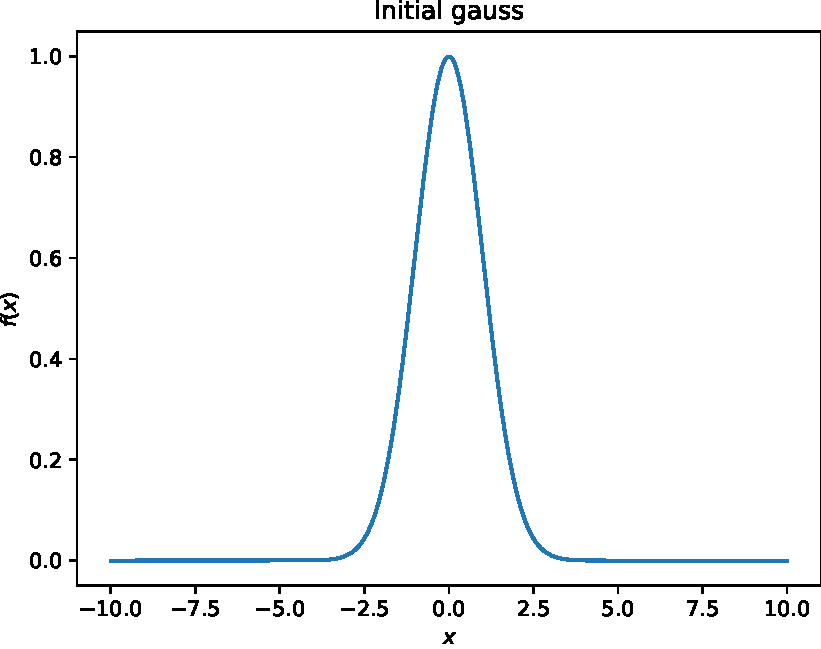
\includegraphics[width=8cm]{pdfs/gauss.pdf}
    \caption{Navadna gausova funkcija}
\end{figure}
Nato jo tranformiramo s pomočjo Furjerjeve transformacije, z mojo lastno implementacijo.
\begin{figure}[h]
    \centering
    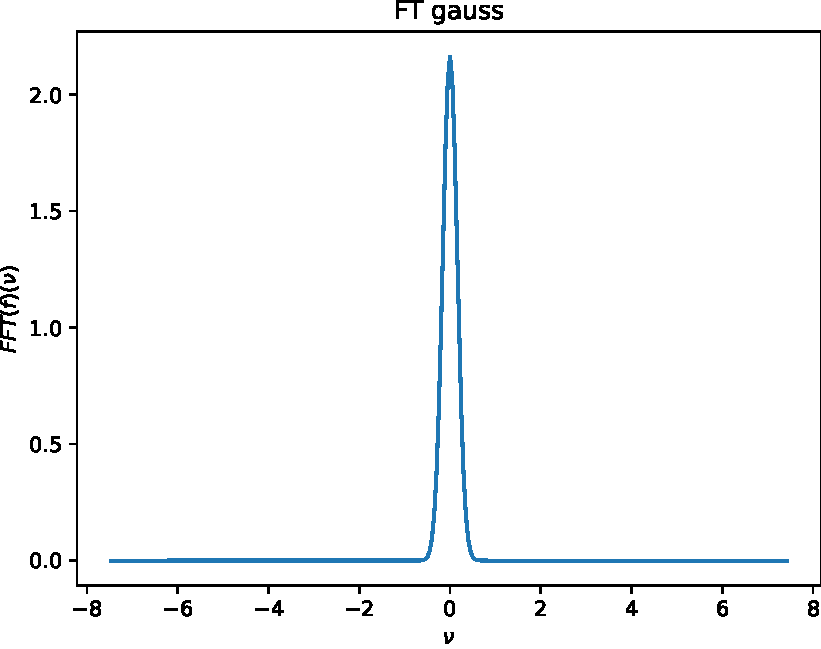
\includegraphics[width=8cm]{pdfs/fft(gauss).pdf}
    \caption{Furjerjeva transformacija navadne gaussove funkcije}
\end{figure}
Po pričakovanjih dobimo spet gaussovko, le malo drugačne oblike. Naredimo še inverzno tranformacijo, da vidimo,
če dobimo spet prvo sliko.
\newpage
\begin{figure}[h]
    \centering
    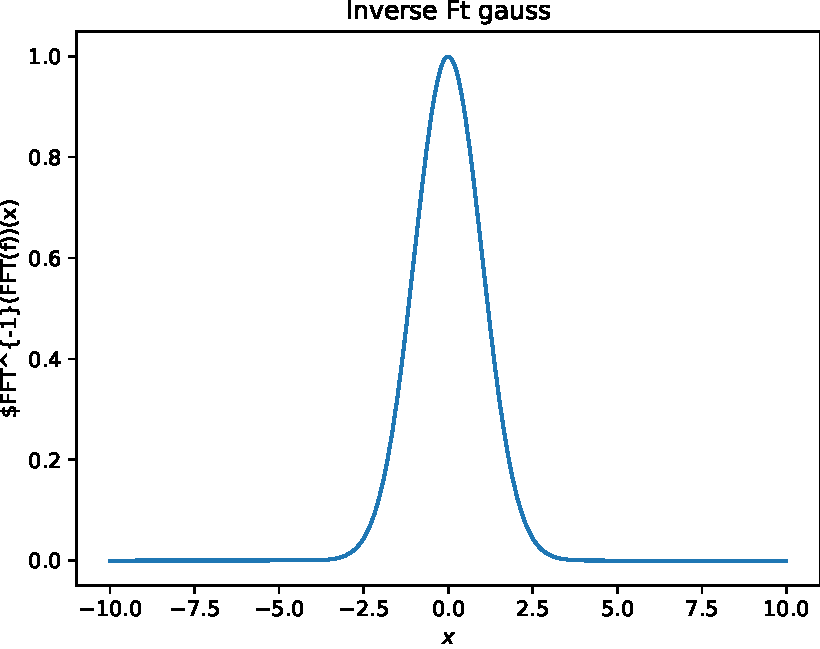
\includegraphics[width=8cm]{pdfs/inf(fft).pdf}
    \caption{Inverz furjerjeve transformacije na gaussovko}
\end{figure}
Poglejmo si še absolutno napako med prvotno sliko in zadnjo, saj iz grafov ne moremo razbrati
dejanske razlike.
\begin{figure}[h]
    \centering
    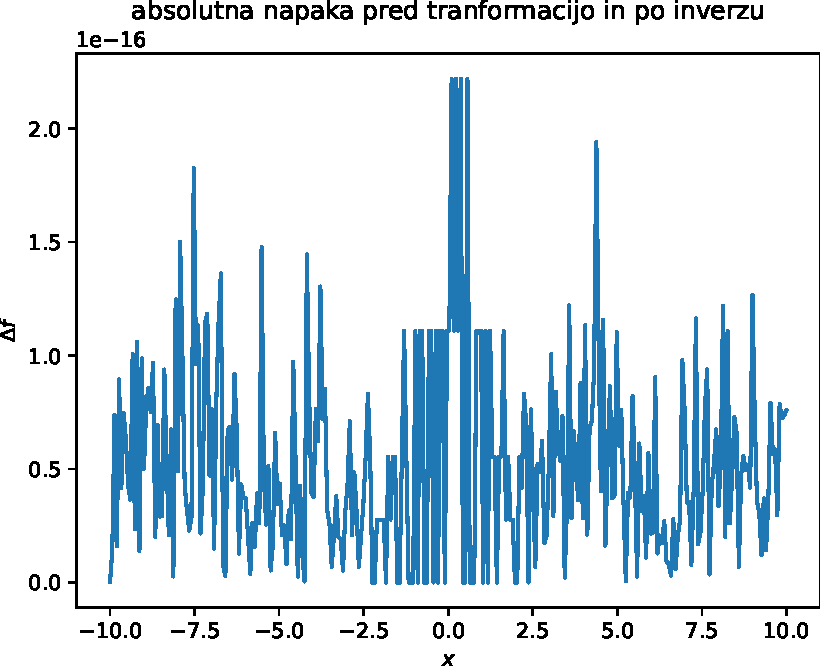
\includegraphics[width=8cm]{pdfs/abs_napaka.pdf}
    \caption{Absolutna napaka po furjerjevi tranformaciji in njenemu inverzu}
\end{figure}
Vidimo, da napaka je zanemarljiva, ker je reda $10^{-16}$.
\newpage
Ker je gaussova funkcija zelo dolgčasna si poglejmo tako funkcijo pri kateri ne zehamo.
\begin{figure}[h]
    \centering
    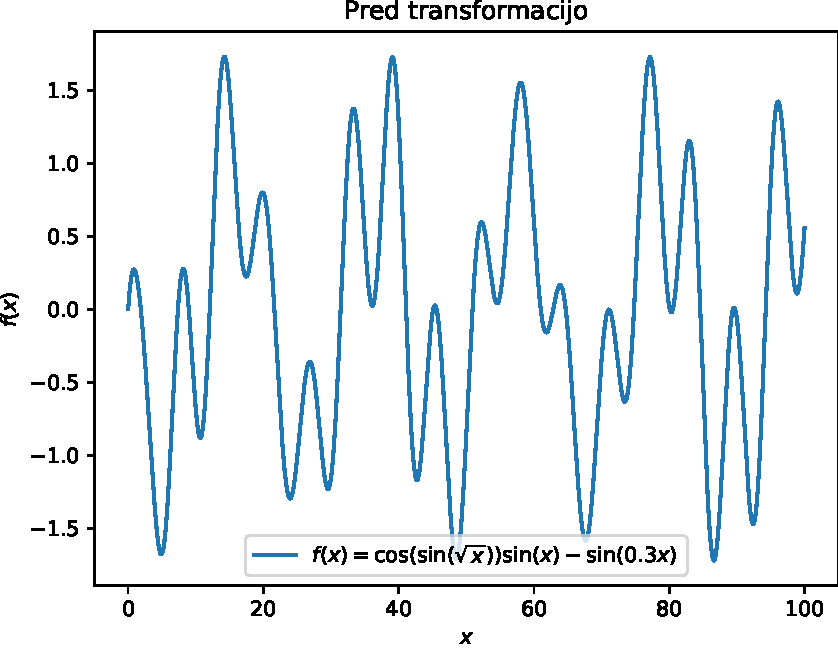
\includegraphics[width=10cm]{pdfs/pred.pdf}
    \caption{Graf funckije $f(x) = \sin(\cos(\sqrt{x}))-\sin(0.3x)$}
\end{figure}
\newpage
\begin{figure}[h]
    \centering
    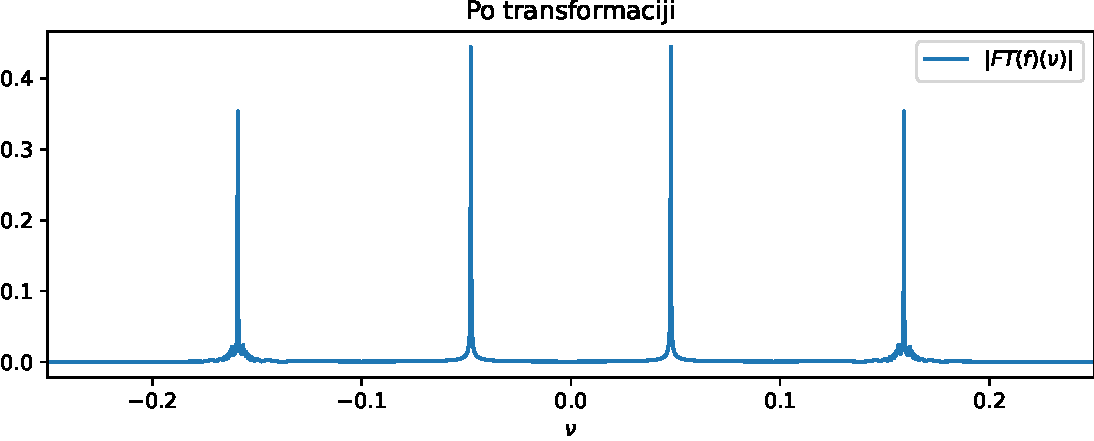
\includegraphics[width=13cm]{pdfs/po.pdf}
    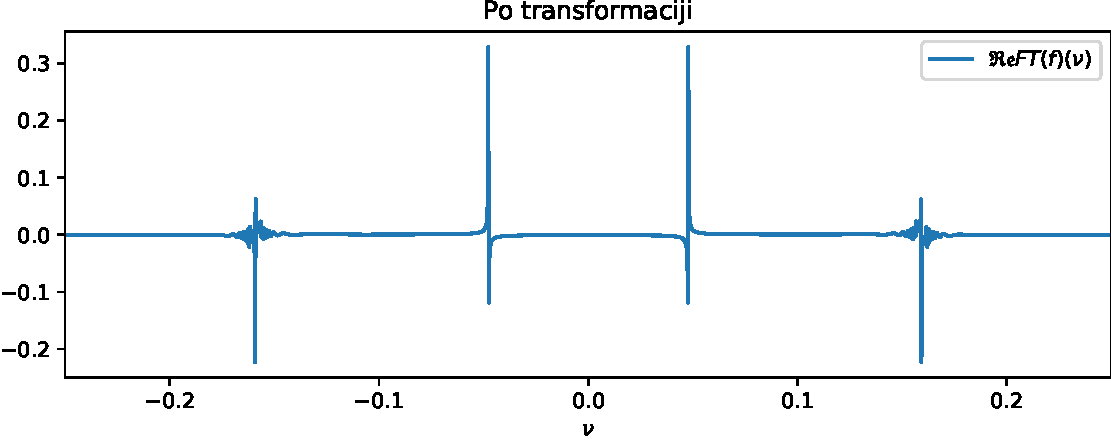
\includegraphics[width=13cm]{pdfs/real.pdf}
    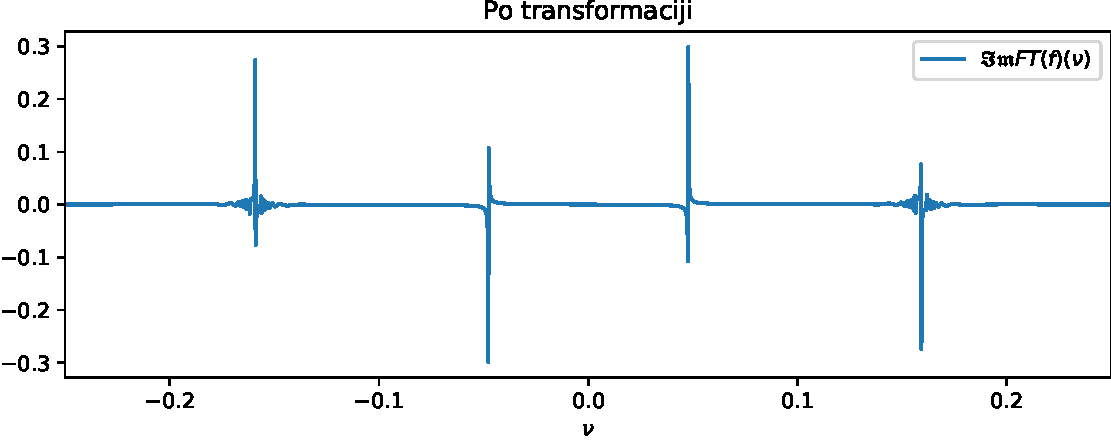
\includegraphics[width=13cm]{pdfs/imag.pdf}    
    \caption{Furjerjeva transformacija funckije $f(x) = \sin(\cos(\sqrt{x}))-\sin(0.3x)$}
\end{figure}
\newpage
Ker imamo dva algoritma enega počasnega enega hitrega, si poglejmo njuno efektivnost, t.p. časovno odvisnost od velikosti vhoda.
\begin{figure}[h]
    \centering
    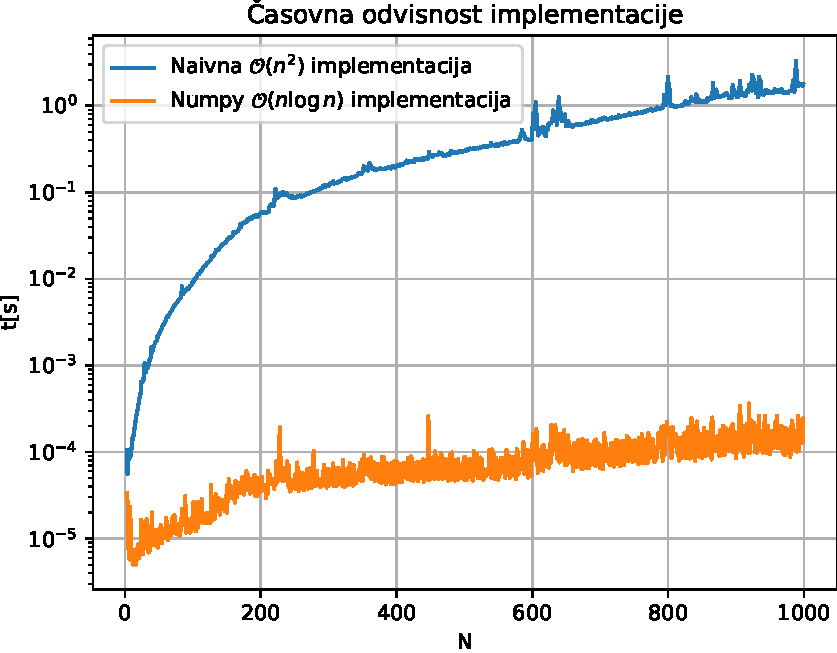
\includegraphics[width=12cm]{pdfs/t(N).pdf}
    \caption{Časovna odvisnost med algoritmoma}
\end{figure}
Moj algoritem deluje v $\mathcal{O}(n^2)$ in je implementiran po definiciji iz navodil,
med tem pa že implementiran \verb|numpy.fft.fft()| deluje $\mathcal{O}(n\log n)$ z malo bolj zvitimi metodami.
\newpage
Poglejmo si še kaj se dogaja pri FT, če imamo vzorčenje blizu nyquistove frekvence.
\begin{figure}[h]
    \centering
    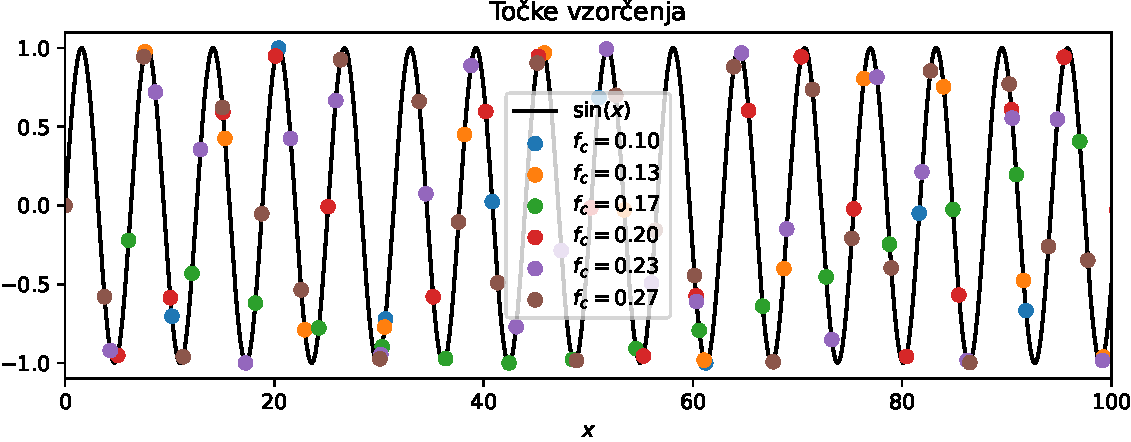
\includegraphics[width=15cm]{pdfs/nyquist.pdf}
    \caption{Vzorčenje točk sinusa}
\end{figure}
Vsaka točka se preslika v svojo krivuljo, kateri ustreza barva. Kot vidimo iz slike se špice premikajo navznozer,
ker so simetrične se pa potem povozijo čez in nato odpotujejo spet malo ven.
\begin{figure}[h]
    \centering
    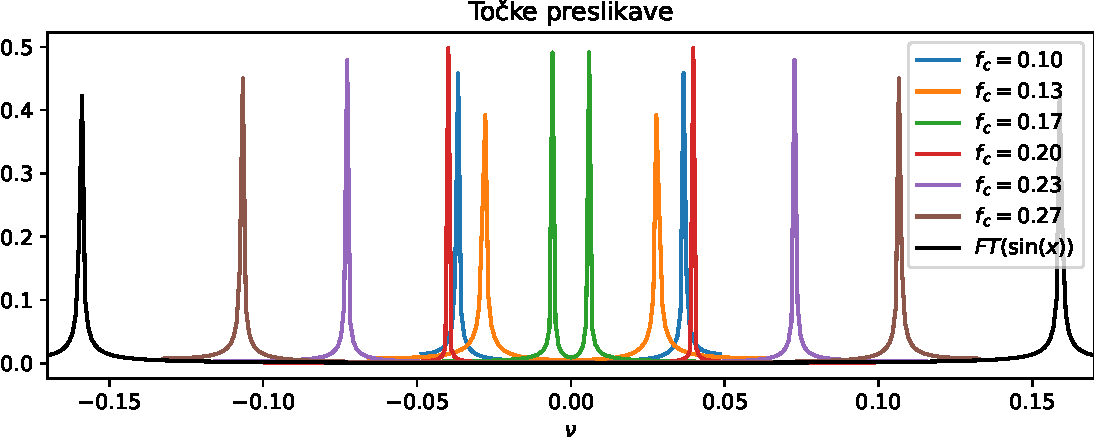
\includegraphics[width=15cm]{pdfs/nyquistfft.pdf}
    \caption{Furjerjeva transformacija vzorčenih točk sinusa}
\end{figure}
\newpage
Poglejmo si še našega Baha, pri različni gostoti vzorčenja (sample-ratih).
\begin{figure}[h]
    \centering
    \foreach \num in {882, 1378, 2756, 5512, 11025, 44100} {
        \includegraphics[width=12cm]{pdfs/\num.pdf}
    }   
    \caption{Absolutna velikost furjerjeve transformacije Bachove skladbe}
\end{figure}
\newpage
\begin{figure}[h]
    \centering
    \foreach \num in {882, 1378, 2756, 5512, 11025, 44100} {
        \includegraphics[width=12cm]{pdfs/\num Re.pdf}
    }   
    \caption{Realna komponenta furjerjeve transformacije Bachove skladbe}
\end{figure}
\newpage
\begin{figure}[h]
    \centering
    \foreach \num in {882, 1378, 2756, 5512, 11025, 44100} {
        \includegraphics[width=12cm]{pdfs/\num Im.pdf}
    }   
    \caption{Imaginarna komponenta furjerjeve transformacije Bachove skladbe}
\end{figure}
\newpage
Kaj pa se dogaja z visokimi frekvencami, ki jih ni slišati zaradi odtujitve. Poglejmo si spektometer.
\begin{figure}[h]
    \centering
    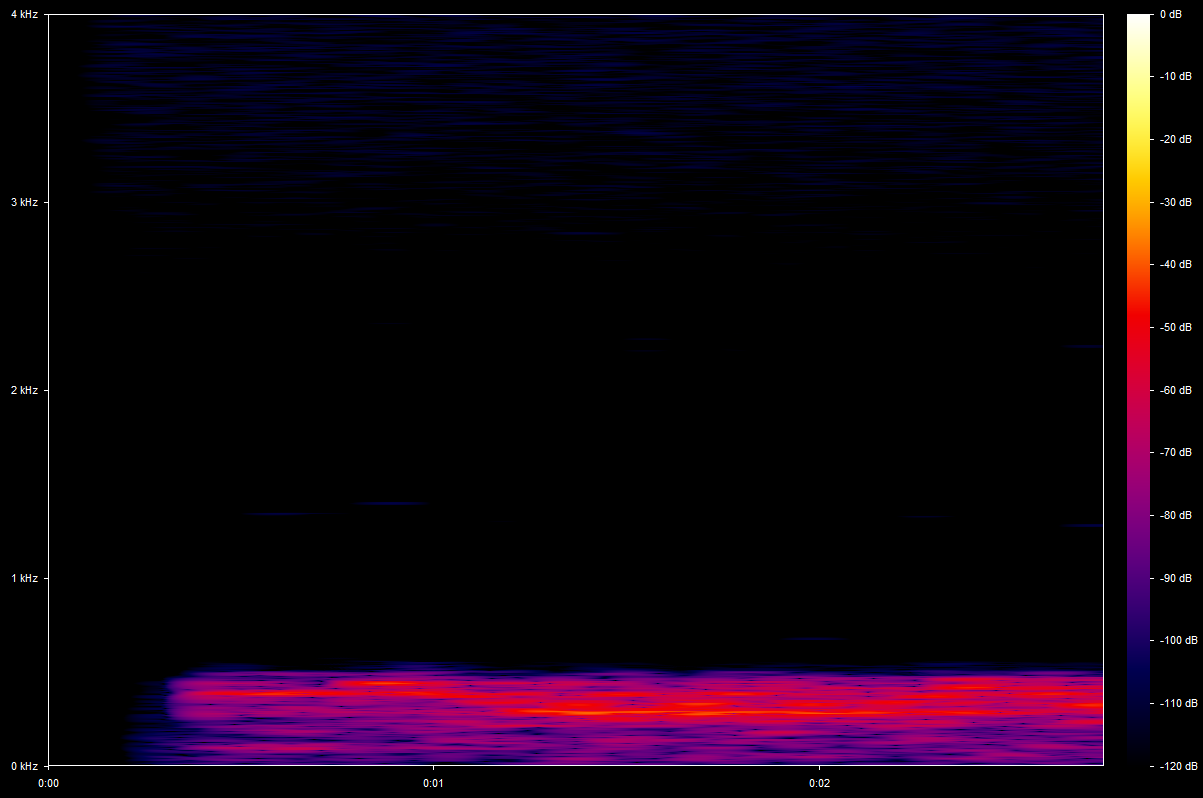
\includegraphics[width=14cm]{pngs/Bach.882.wav.png}
    \caption{Spekter za gostoto vzorčenja 882Hz}
\end{figure}
\newpage
\begin{figure}[h]
    \centering
    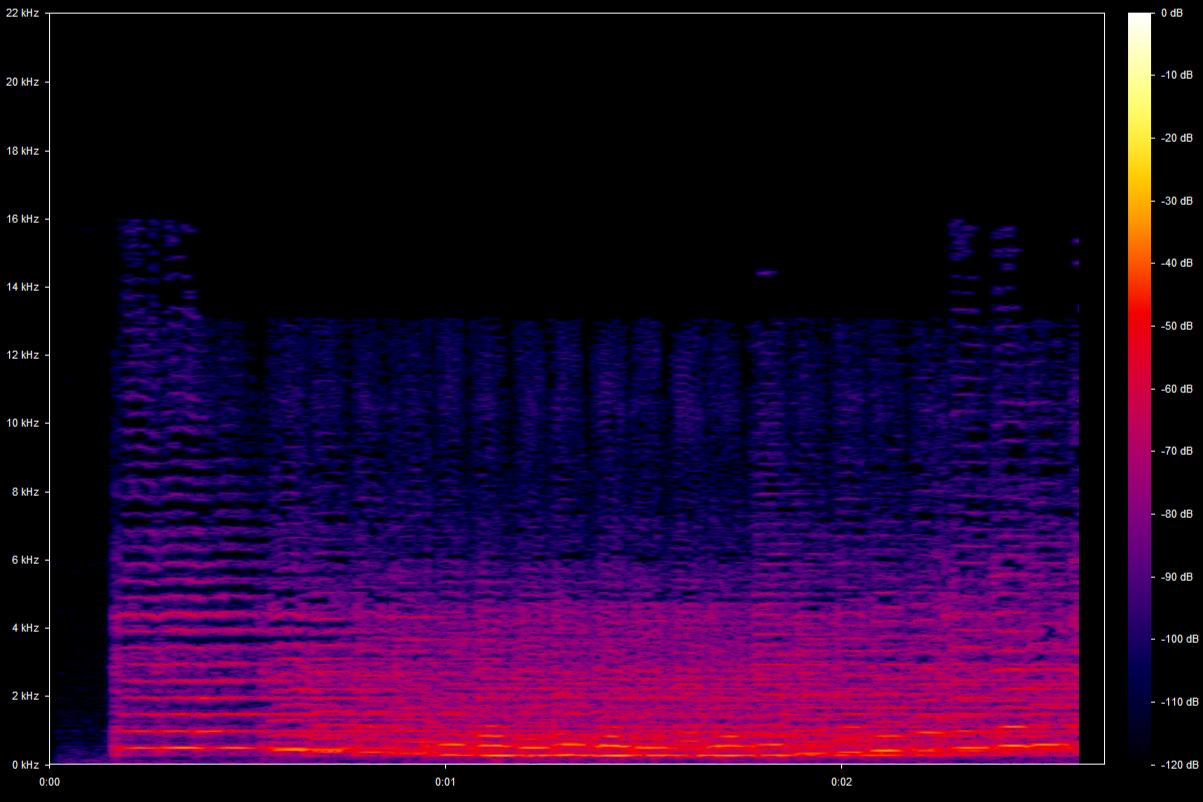
\includegraphics[width=14cm]{pngs/Bach.44100.mp3.png}
    \caption{Spekter za gostoto vzorčenja 44100Hz}
\end{figure}
Vidimo, da nad polovično frekvenco vzorčenja, ni signala.